\chapter{Frameworks, Libraries and software tools} \label{chap:lib}

As explained previously, the core of the design is the use of the SEcube™ chip as device to perform security operations in order to encrypt/decrypt some data stored in the host (PC). The requests to the device are made from the C/C++/Qt application developed in this work, which runs in the host machine. Said application exploits the existing C libraries SEfile and secureSQLite from the SEcube™ framework to ease the communication with the device. The chip firmware, written in C, is done using the Eclipse IDE. Additionally, the application uses of the random password generator PwGen and the password strength estimator zxcvbn, both of them open source libraries. A passphrase generator function was also developed and to keep some order it is treated as a library.

In the following sections a review of the SEcube™ platform's hardware and software components is given. Then a brief explanation of the C/C++/Qt framework and why it was chosen. Finally the additional software tools and libraries are presented.

\section{The SEcube™ framework}

``The SEcube™ (Secure Environment cube) Open Security Platform is an open source security oriented hardware and software platform, designed and constructed with ease of integration and service-orientation in mind. The hardware part of the platform was originally designed by Blu5 Group \cite{Blu5}, whereas the software libraries stem from a strong cooperation among international research institutions.'' \cite{GetStart}.

\vspace{5pt}

The main \textbf{hardware} products, explained in detail in the following sections, are:
\begin{itemize}
\setlength\itemsep{0pt}
\item The Chip, named SEcube™ Chip, or simply \textbf{SEcube™}
\item The Development Board, named \textbf{SEcube™ DevKit}
\item The USB Stick, named \textbf{USEcube Stick}.
\end{itemize}

The SEcube™ chip is the main hardware component, and both the devkit and USB Stick are designed around it.The Development Board provides several communication protocols as well as debugging capabilities. For the final product the board would be of course too inconvenient to carry, and instead the USEcube Stick is preferred.

\subsection{The SEcube™ Chip}

``The SEcube™ (Secure Environment cube) is a powerful chip which
integrates three key security elements in a single package. A fast
floating-point Cortex-M4 \textbf{CPU}, a high-performance \textbf{FPGA} and an
EAL5+ certified Security Controller (\textbf{Smart Card}).
The result of this innovative combination gives an extremely
versatile secure environment in a single SoC, in which developers
can rapidly implement complex applications and appliances.
... The SEcube™ is the ultimate solution for high-end design,
delivering integration of a flexible, configurable and certified
secure element.'' \cite{SEcubeDS}

We can then see the SEcube™ chip as a powerful device offering the flexibility of an \textsc{ARM} CPU, the speed of an FPGA and the reliable security of a certified Smart Card, all bounded together and easily integrated in any project thanks to the available communication protocols, among them USB, UART, Ethernet and JTAG. 

The chip includes a true random number generator which relies in 240 noise seeds, all physical and therefore unpredictable. This allows the creation of true random noise. Additionally the user can choose what type of noise they want to generate, for instance white or Fourier noise.

%TODO
\todo{talk more about cpu, low power modes...}

In figure \ref{fig:SEcubeBD} a simplified SEcube™ architecture is shown.

\begin{figure}[ht]
	\centering
	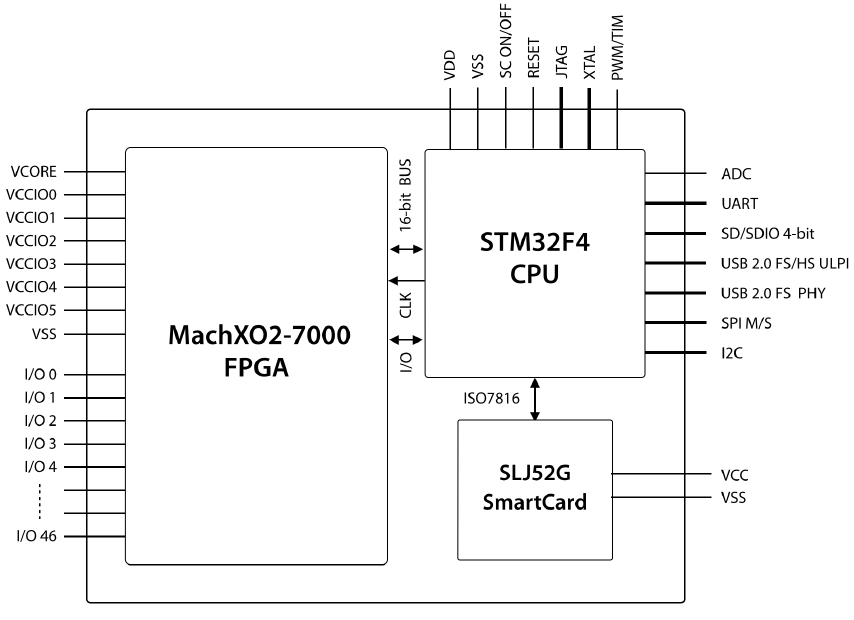
\includegraphics[width=\textwidth]{chapters/figures/development/SEcubeBlocks.png}
	\caption{SEcube™ Block Diagram}
	\label{fig:SEcubeBD}
\end{figure}


\subsection{Development board: The SEcube™ DevKit}

The development board integrates the SEcube™ chip with several peripherals that allow the user to easily communicate, program and debug. (Figure \ref{fig:devboard})

\begin{figure}[ht]
  \centering
  \subfloat[]{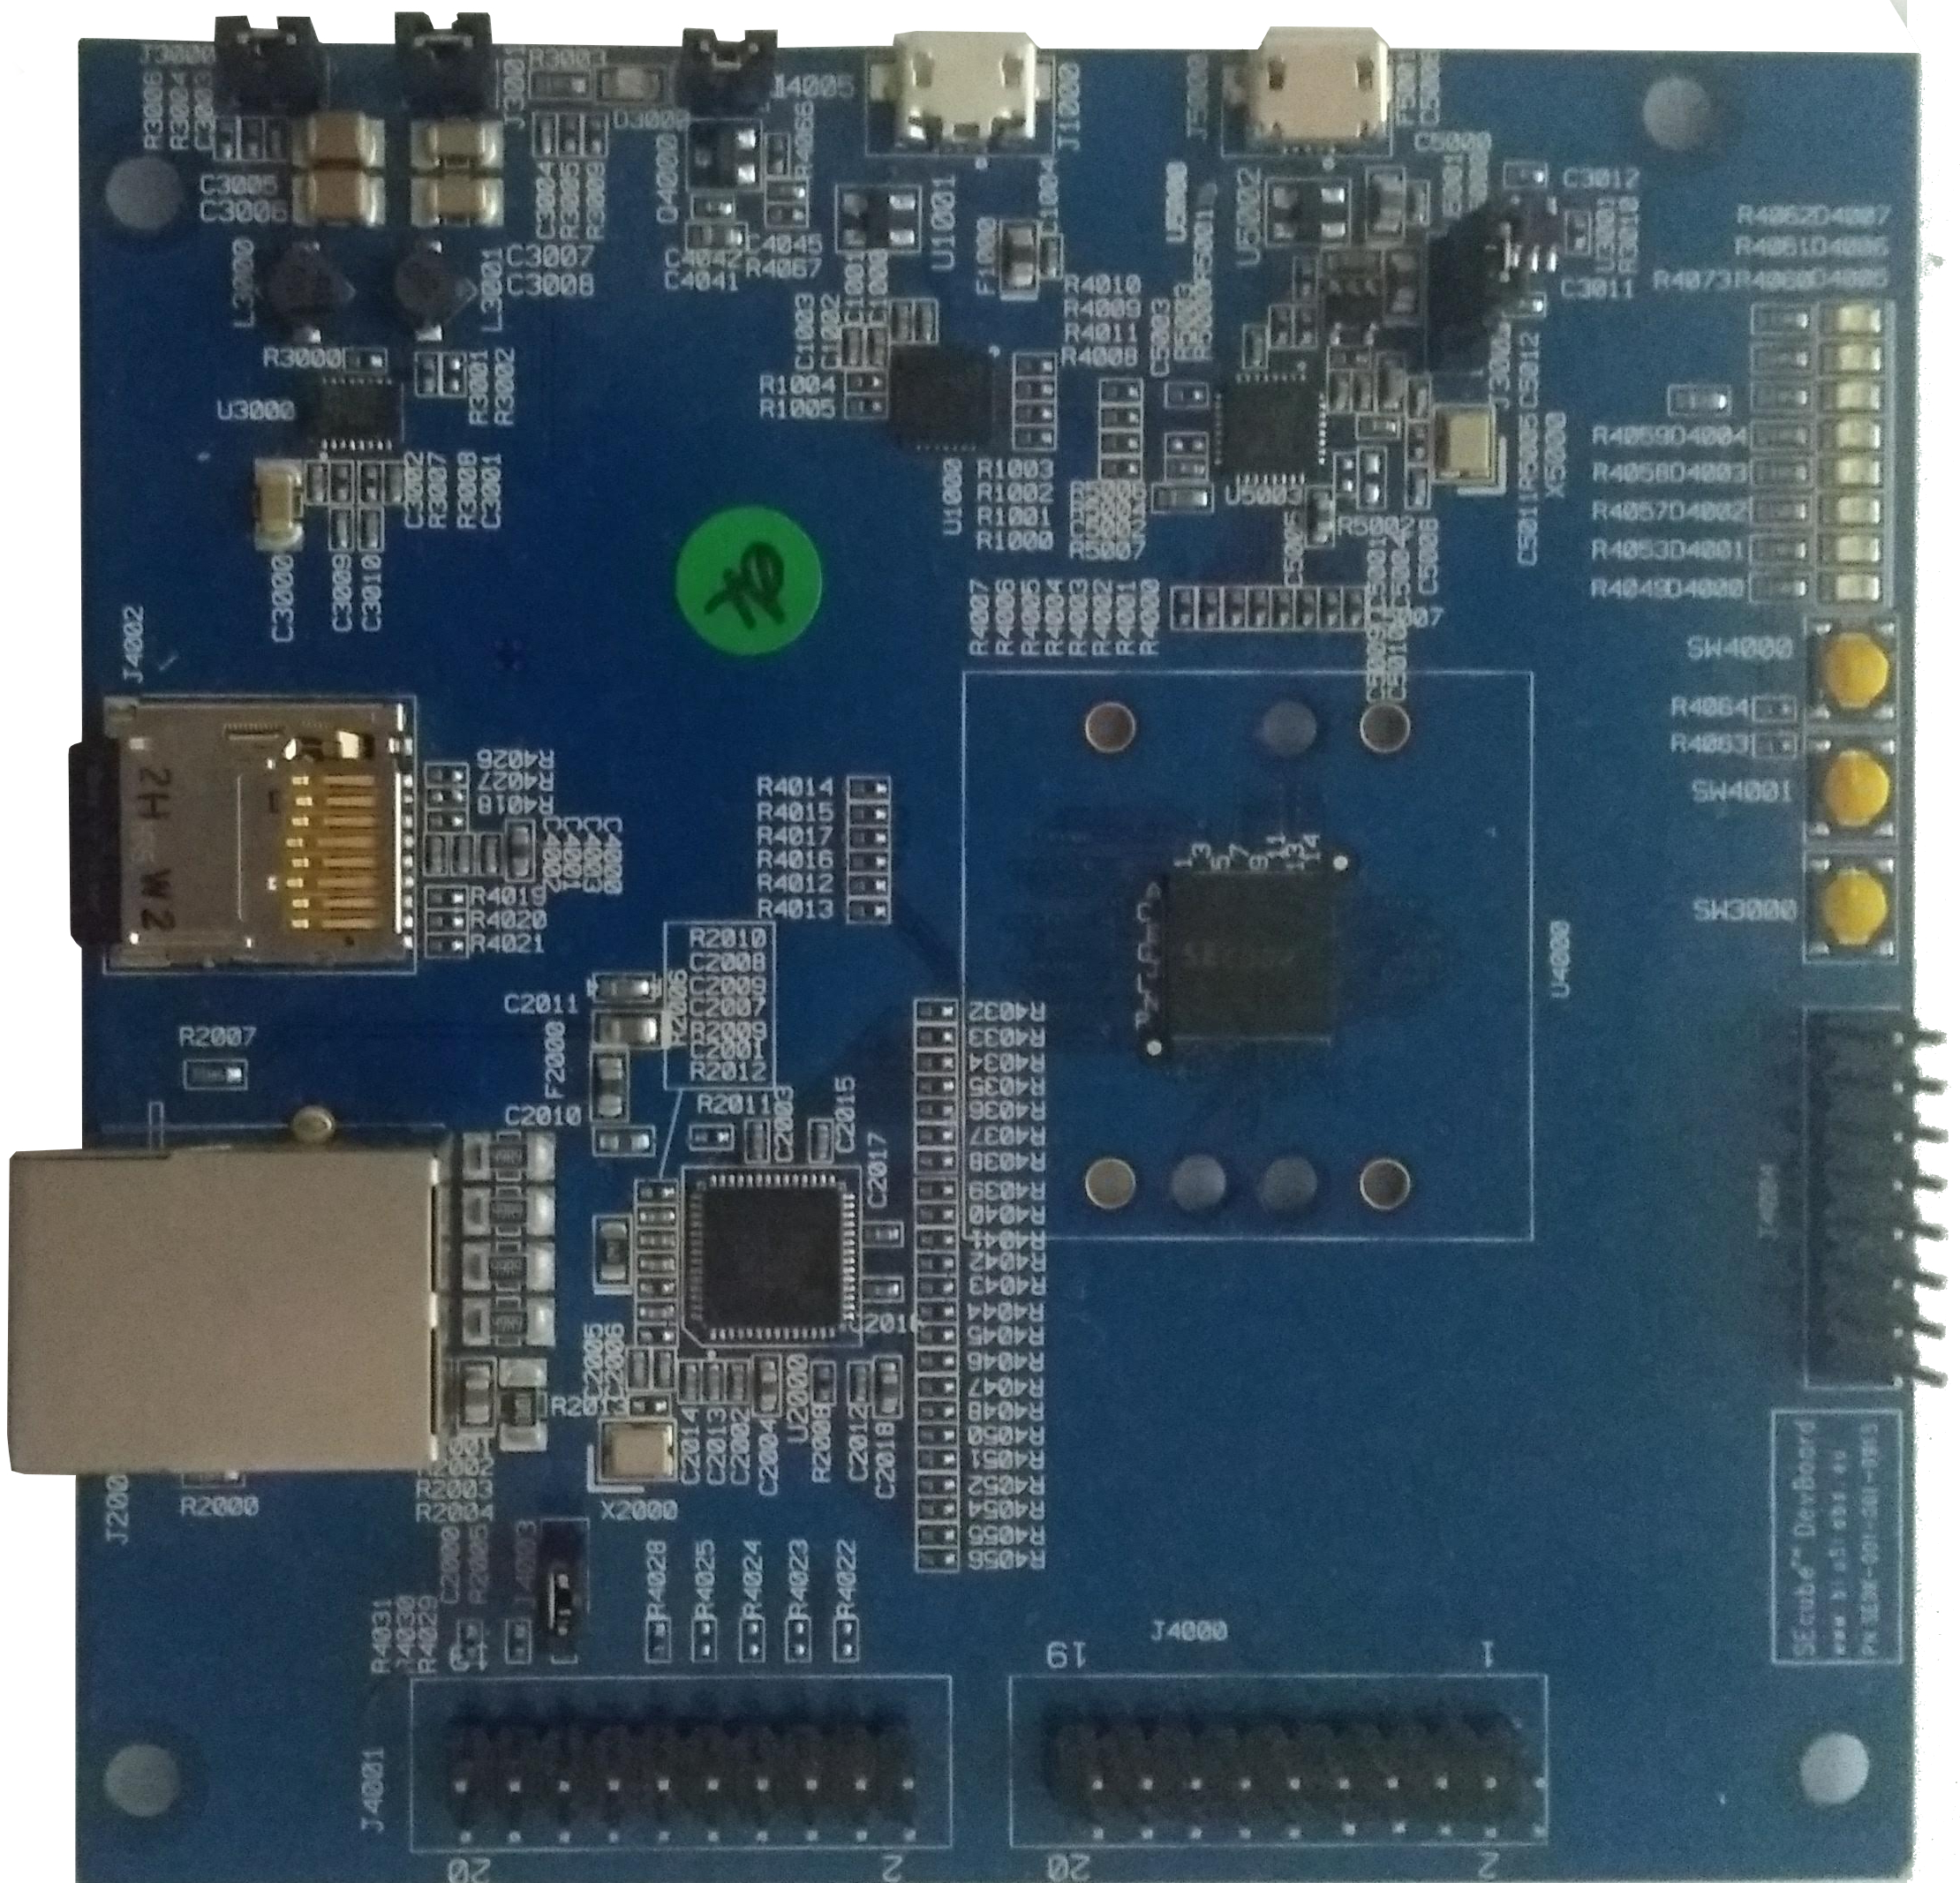
\includegraphics[width=0.485\textwidth]{chapters/figures/development/devboard.jpg}}
  \subfloat[]{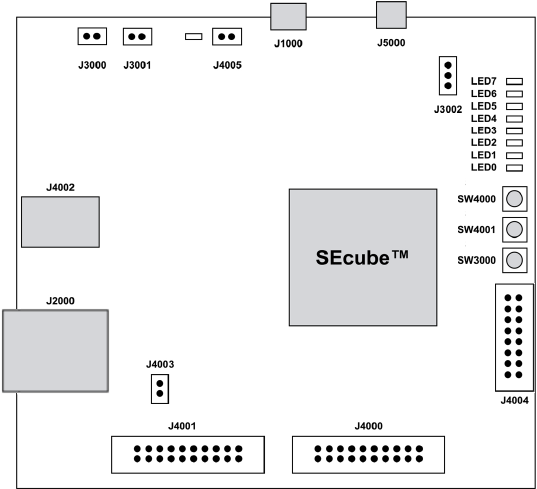
\includegraphics[width=0.515\textwidth]{chapters/figures/development/devboard_sch.png}}
  \caption{SEcube™ Devkit}
 \label{fig:devboard}
\end{figure}

The main peripherals in the SEcube™ devkit are:

\begin{itemize}
\setlength\itemsep{-3pt}
\item \textbf{J1000: }\tabto{2.3cm} USB 2.0 to UART 
\item \textbf{J2000: }\tabto{2.3cm} Ethernet 10/100 socket 
\item \textbf{J4000: }\tabto{2.3cm} SEcube™ embedded FPGA and CPU GPIOs
\item \textbf{J4001: }\tabto{2.3cm} SEcube™ embedded CPU JTAG
\item \textbf{J4002: }\tabto{2.3cm} microSD card 
\item \textbf{J4004: }\tabto{2.3cm} SEcube™ embedded FPGA and CPU GPIOs
\item \textbf{J5000: }\tabto{2.3cm} USB 2.0 High Speed 
\item \textbf{LEDx:  }\tabto{2.3cm} Leds 
\item \textbf{SWx00y:}\tabto{2.3cm} Switches 
\end{itemize}

\subsection{Final product: USEcube Stick}

For the final product, its is desired that the user carries all the SEcube™ functionalities in a small and convenient package, so they can encrypt/decrypt the passwords in any PC by just connecting the USEcube Stick and running the SEcubeWallet application.

The USEcube Stick is compatible with any Operating System and the SEcube™ functionalities are easily exposed to applications and services without installing any driver.

The USEcube offers only the strictly required components: The SEcube™ chip, a USB 2.0 High-Speed interface and an SDcard socket. See Figure \ref{fig:USEcube} for more details.


Since the USEcube Stick storage capability is based on a external microSD card, the security of the system is improved, as this allows to have a separation of encrypted data from the encryptor/decryptor. Additionally, both the size and the speed can be tuned per the user requirement and can be changed at any time, just replacing the microSD, without buying a new USEcube Stick.
The microSD card socket is embedded in the USB connector allowing to save space making the USEcube Stick very compact and, at the same time dust
and water-resistant.
Since the USEcube Stick is not provided with the JTAG interface, to inject the firmware previously developed and tested on the SEcube™ DevKit, all the devices come with an embedded secure boot loader.


\begin{figure}[ht]
  \centering
  \subfloat[]{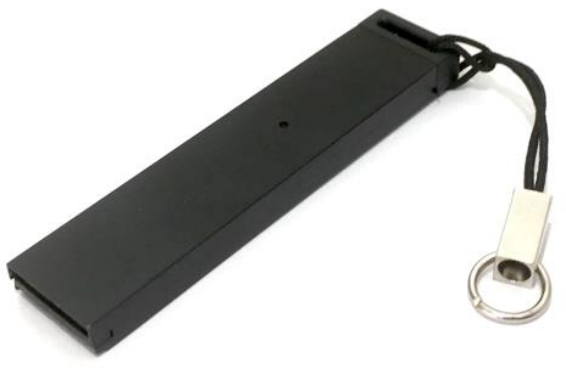
\includegraphics[width=0.485\textwidth]{chapters/figures/development/usb.png}}
  \subfloat[]{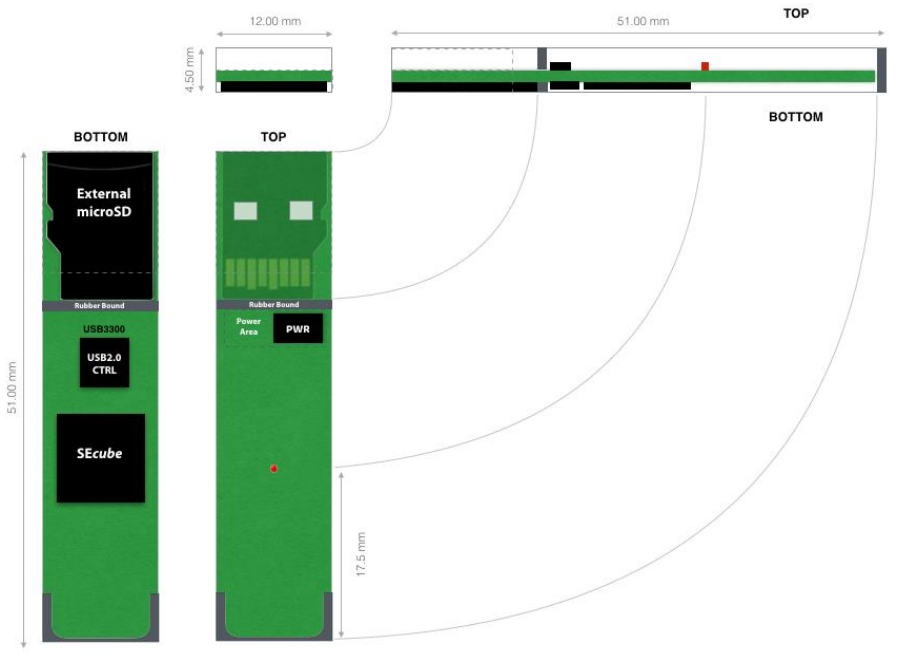
\includegraphics[width=0.515\textwidth]{chapters/figures/development/usb_sch.png}}
  \caption{USEcube Stick}
 \label{fig:USEcube}
\end{figure}

\subsection{SEcube™ Open SDK}

The SEcube™ Open SDK available at \cite{SEcubeRes} is a set of libraries, for both the SEcube™ device and the host machine. In general, the user interacts with the host libraries requesting security services. The host in turn pass those request to the device libraries, which are the ones that actually execute any security algorithms. The results are passed back to the host and ultimately to the user.

``The software libraries and design environment allow developers who are not willing or able to produce the security APIs and protocols themselves to exploit the ready functions provided (currently as APIs and soon as services) within the SEcube™ platform and experience the platform as a high-security black box.'' \cite{L2UserMan}

``From the user/developer point of view, the APIs have been implemented targeting two
nested environments depending on where physically the code runs:
\begin{itemize}
\setlength\itemsep{1pt}
\item \textbf{Device-Side}, including the libraries of basic functionalities that are executed on the embedded processor of the SEcube™-based hardware device.
\item \textbf{Host-Side}, containing libraries of functions executed on the host PC and interface functions for calling services and processes residing on the embedded processor of the SEcube™ device.
\end{itemize} 

From the architectural point of view, the Host-Side Libraries have been implemented targeting 4 hierarchical abstraction levels, and namely:
\begin{itemize}
\setlength\itemsep{-3pt}
\item \textbf{Level 0:} Communication Protocol and Provisioning APIs
\item \textbf{Level 1:} Basic Security APIs
\item \textbf{Level 2:} Intermediate Security APIs
\item \textbf{Level 3:} Advanced Security APIs
\end{itemize}

At each level, each component represents a "service" for the upper level and relies on "services" provided by the next lower level, only.'' \cite{L2UserMan}

The Device-Side Libraries only have the lower two levels of abstraction, and each of these levels communicates with its host-side counterpart.

In Figure \ref{fig:levels} a graphical representation of the hierarchical levels is presented. For each level is shown, in parenthesis, an example of a function/application belonging to it.

\begin{figure}[htb]
  \centering
  \captionsetup{justification=centering}
  \centerline{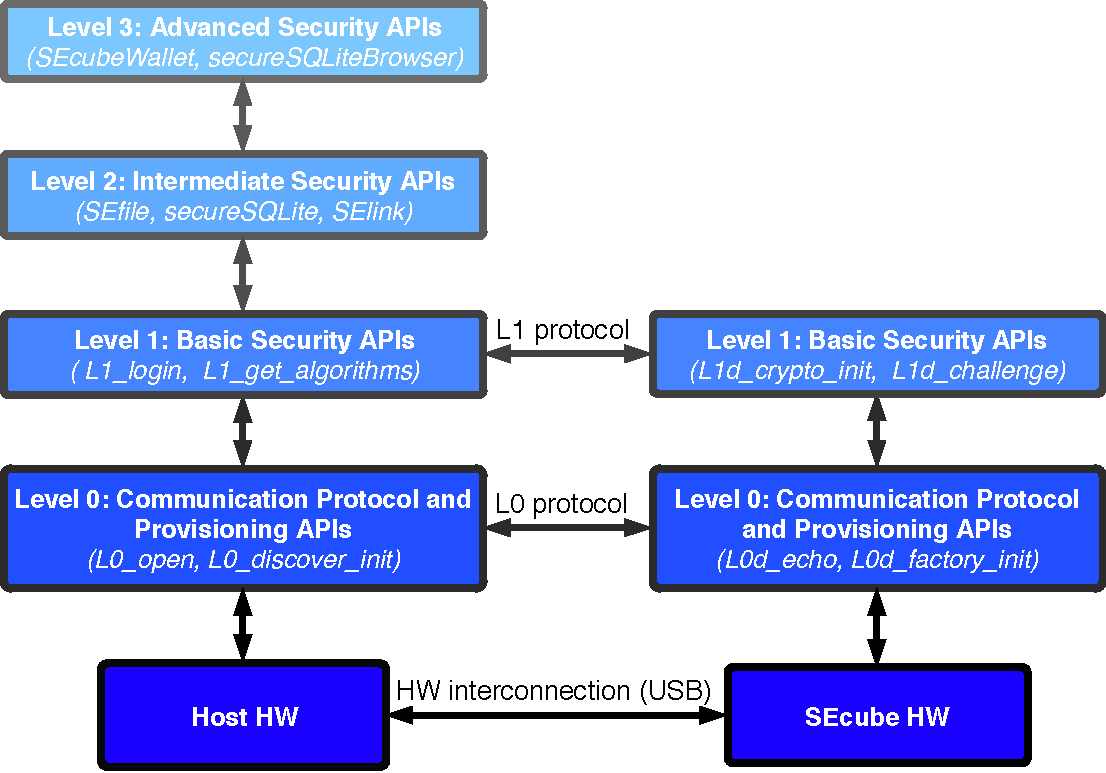
\includegraphics[width=\columnwidth]{chapters/figures/frameworks/levels.pdf}}
  \caption{Libraries Hierarchy Levels}
  \label{fig:levels}
\end{figure}

\subsection{Level 2: Intermediate Security APIs}

SEcubeWallet is a Level 3 application that relies heavily on the Level 2 APIs SEfile and secureSQLite. In this section a review of these APIs is given.

``Level L2 relies on L1 services to provide the APIs for implementing more abstract secure functionalities. Typical examples include APIs for the protection of data both at rest and in-motion, or negotiating parameters (e.g., keys, algorithms) for establishing secure sessions, without being forced to understand in details all the low-level hardware and security mechanisms.''\cite{L2UserMan}

L2 can be considered as the merge of two projects: \textbf{SEfile}, concerning data at rest, and \textbf{SElink}, concerning instead data at motion. 

\subsection{SEfile}

``SEfile targets any user that, by moving inside a secure environment, wants to perform basic operation on regular files. It must be pointed out that all encryption functionalities are demanded to the secure device in their entirety. In addition, SEfile does not expose to the host device details about what, or where it is reading/writing data: thus, the host OS, which might be untrusted, is totally unaware of what it is writing''. \cite{L2UserMan}.


A secured file has the structure shown in figure \ref{fig:secfile}. The data is divided in sectors, and each of them is encrypted and signed. The first sector does not contain data, but metadata on the file itself, and it is known as the header.

When a portion of the file wants to be read or written (i.e. encrypted or decrypted), it is not necessary to process the whole file. Only the required sectors are manipulated, thus reducing the overhead time of securing operations.

\begin{figure}[htb]
  \centering
  \captionsetup{justification=centering}
  \centerline{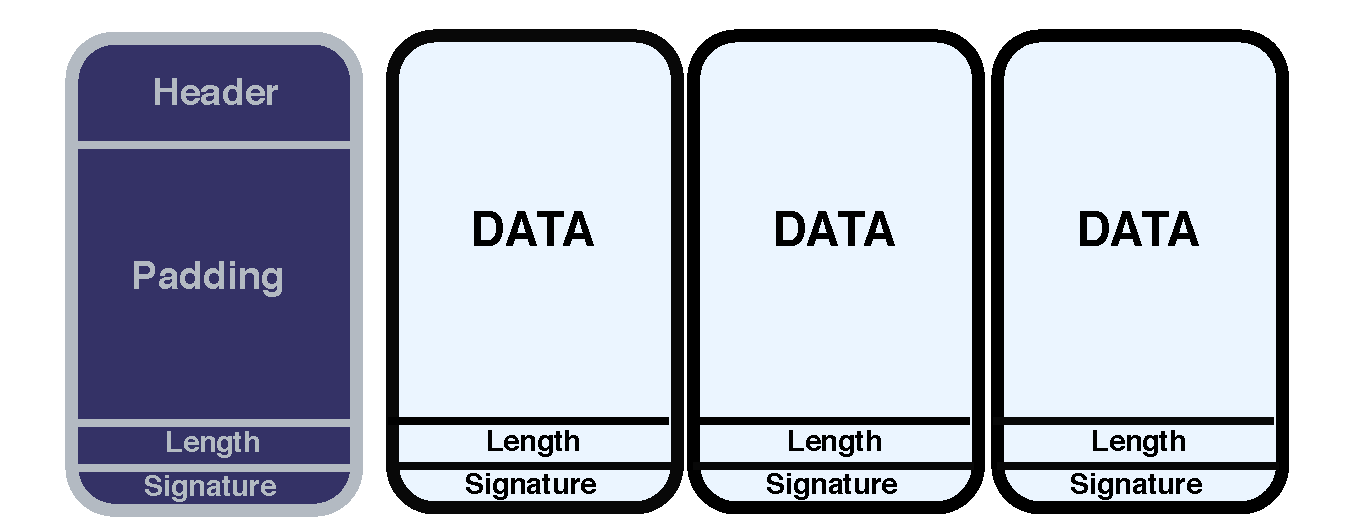
\includegraphics[width=1\columnwidth]{chapters/figures/frameworks/secfile.pdf}}
  \caption{Secure File structure}
  \label{fig:secfile}
\end{figure}

For file encryption, SEfile uses The Advanced Encryption Standard (AES), established by the U.S. National Institute of Standards and Technology (NIST). For each data sector AES-256-CTR is used, while the header sector is encrypted using AES-256-ECB.

For authentication, ``each sector, including the header, is signed using an authenticated signature obtained with SHA-256-HMAC, meaning that the signature depends on both the data contained in the sector itself and on a chosen encryption key. To use two different keys to encrypt data and to digest authentication, a feature increasing overall system security, SEfile leverages on the pbkdf2() function already implemented within the SDK.''\cite{L2UserMan}


\subsection{secureSQLite}

Based on the SQLite data base management system, and using SEfile, this API allows the user to create SEcube™ secured data bases.
``Leveraging on its modularity, the SQLite system has been modified to resort on a custom functionalities wrapper based on SEfile, rather than using directly the OS calls. The starting point of this work was the template offered as example for making a custom VFS interface distributed along with SQLite, version 3.13.0.''\cite{L2UserMan}

Every database created with secureSQLite is cyphered and signed up to its file name before being stored, thus making it impossible to read the database contents without authenticating and using the library.

\section{SQLite Data Base management system}
A Data Base is a structured set of data stored and accessed electronically using a data base management system. 

SQLite \cite{SQLite} is one of such management systems. It implements most of the SQL (Structured Query Language) standard. Unlike most other SQL databases, it is serverless, meaning there is not separate server process, and an application can access directly the database file without the need of interprocess communication. SQLite is ACID (Atomicity, Consistency, Isolation, Durability) compliant, meaning database transactions are valid even in case of errors, leading to program crashes, OS crashes or power failures. It can run in any operating system, even embedded ones. SQLite is implemented in generic C, and it is self-contained in a C library, meaning it has very few dependencies and all the code is encapsulated single source code file. 

In this work the Qt SQLite plugin was used to manage the in-memory SQLite databases. ``The Qt SQLite plugin makes it possible to access SQLite databases\dots SQLite operates on a single file, which must be set as the database name when opening a connection. If the file does not exist, SQLite will try to create it. SQLite also supports in-memory and temporary databases. Simply pass respectively ":memory:" or an empty string as the database name.'' \cite{qsqlite}.

\section{Graphical User Interface: the Qt framework}
The application's graphical user interface was developed using the \textbf{Qt framework}, version 5.11.1, available for download at \cite{qtdown}. (Qt 5.10 or higher is required to compile the sources of this project, as it uses the \texttt{QRandomGenerator} Class included in that version).

``Qt is a cross-platform application development framework for desktop, embedded and mobile. Supported Platforms include Linux, OS X, Windows, VxWorks, QNX, Android, iOS, BlackBerry, Sailfish OS and others. Qt is not a programming language on its own. It is a framework written in C++. A preprocessor, the MOC (Meta-Object Compiler), is used to extend the C++ language with features like signals and slots. Before the compilation step, the MOC parses the source files written in Qt-extended C++ and generates standard compliant C++ sources from them. Thus the framework itself and applications/libraries using it can be compiled by any standard compliant C++ compiler like Clang, GCC, ICC, MinGW and MSVC''.\cite{Qt}  


For writing, compiling and debugging source code, the IDE \textbf{Qt Creator}, version 4.6.2 was used.

``Qt Creator provides a cross-platform, complete integrated development environment (IDE) for application developers to create applications for multiple desktop, embedded, and mobile device platforms, such as Android and iOS. It is available for Linux, macOS and Windows operating systems''.\cite{QtC}.

\vspace{5pt}
The reasons behind the use of Qt are as follows:

\begin{itemize}
\setlength\itemsep{0pt}
\item Qt is a C++ library, and as such, allows for a seamless use of the C libraries SEfile and secureSQLite, which are the backbone of this project.

\item Qt is cross-platform, meaning the developed application can be compiled to work on any of the major OSes. In particular, the development was carried out an tested on a Linux machine, but the application should work with no problems in Windows and MacOS. 

\item Because of good designed and ready-to-use display items such as tables, menus and dialogues, it is possible to focus in writing the functional portions of the application without worrying too much about the GUI. And as it is open source, any Qt item can be modified and extended when it does not meet the expectations out of the box. In this project several display elements were improved, as will be seen in section \ref{sec:imp}.

\item Thanks to the multitude of functions dedicated to ease the use of C++ libraries and OS calls, one can be more productive, and the resulting code is more reliable. For instance, this project makes extensive use of such libraries, like QSqlDatabase, QString, QProcess, etc. Again, more details are given in section \ref{sec:imp}

\item The Related works described in section \ref{sec:relsecube}, secureSQLiteBrowser, SEfile\_TXT and SEfile\_IMG, are written in Qt.

\item Qt is widely used, meaning it is possible to find tons of documentation, forums and additional libraries on the web. This also ensures the Qt framework will have continuous support from the developers and the community.

\end{itemize}

\section{Device side development: Eclipse}

For device-side development, the Eclipse IDE for C/C++, version Neon.3 Release (4.6.3) \cite{eclipse} was used. 

Although this thesis work regards mostly host-side code development (i.e. the Qt application SEcubeWallet), it was necessary to do some slight modifications to the firmware running in the SEcube™ chip, as will be explained in details in section \ref{sec:authen}. 

Eclipse is the recommended IDE for SEcube™ firmware development, as stated in the Getting Started guide \cite{GetStart}. With Eclipse it is possible to perform all the operations required to effectively modify the code running inside the SEcube™ chip, namely write/modify the code, compile it, load it into the chip, and if necessary debug it. But because the code will run in an embedded system, more specifically in an ARM microprocessor, some additional tools and plugins are needed. 

In order to program and debug the chip, an ST-Link/V2 was used. The ST-Link/V2 is an professional tool to debug and program STM8 and STM32 MCUs. It communicates with the microcontroller using the JTAG/SWD connection present in the DevKit board, as see in figure \ref{fig:con}

\begin{figure}[ht]
  \centering
  \subfloat[]{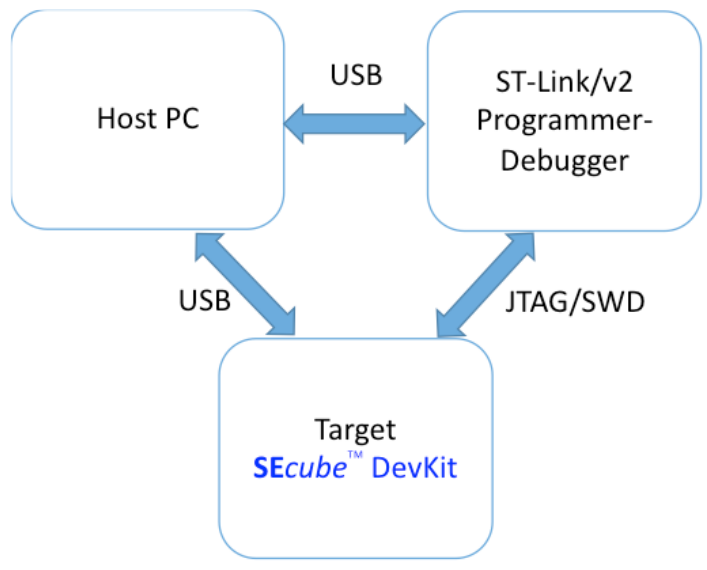
\includegraphics[width=0.48\textwidth]{chapters/figures/frameworks/conSche}}
  {}
  \subfloat[]{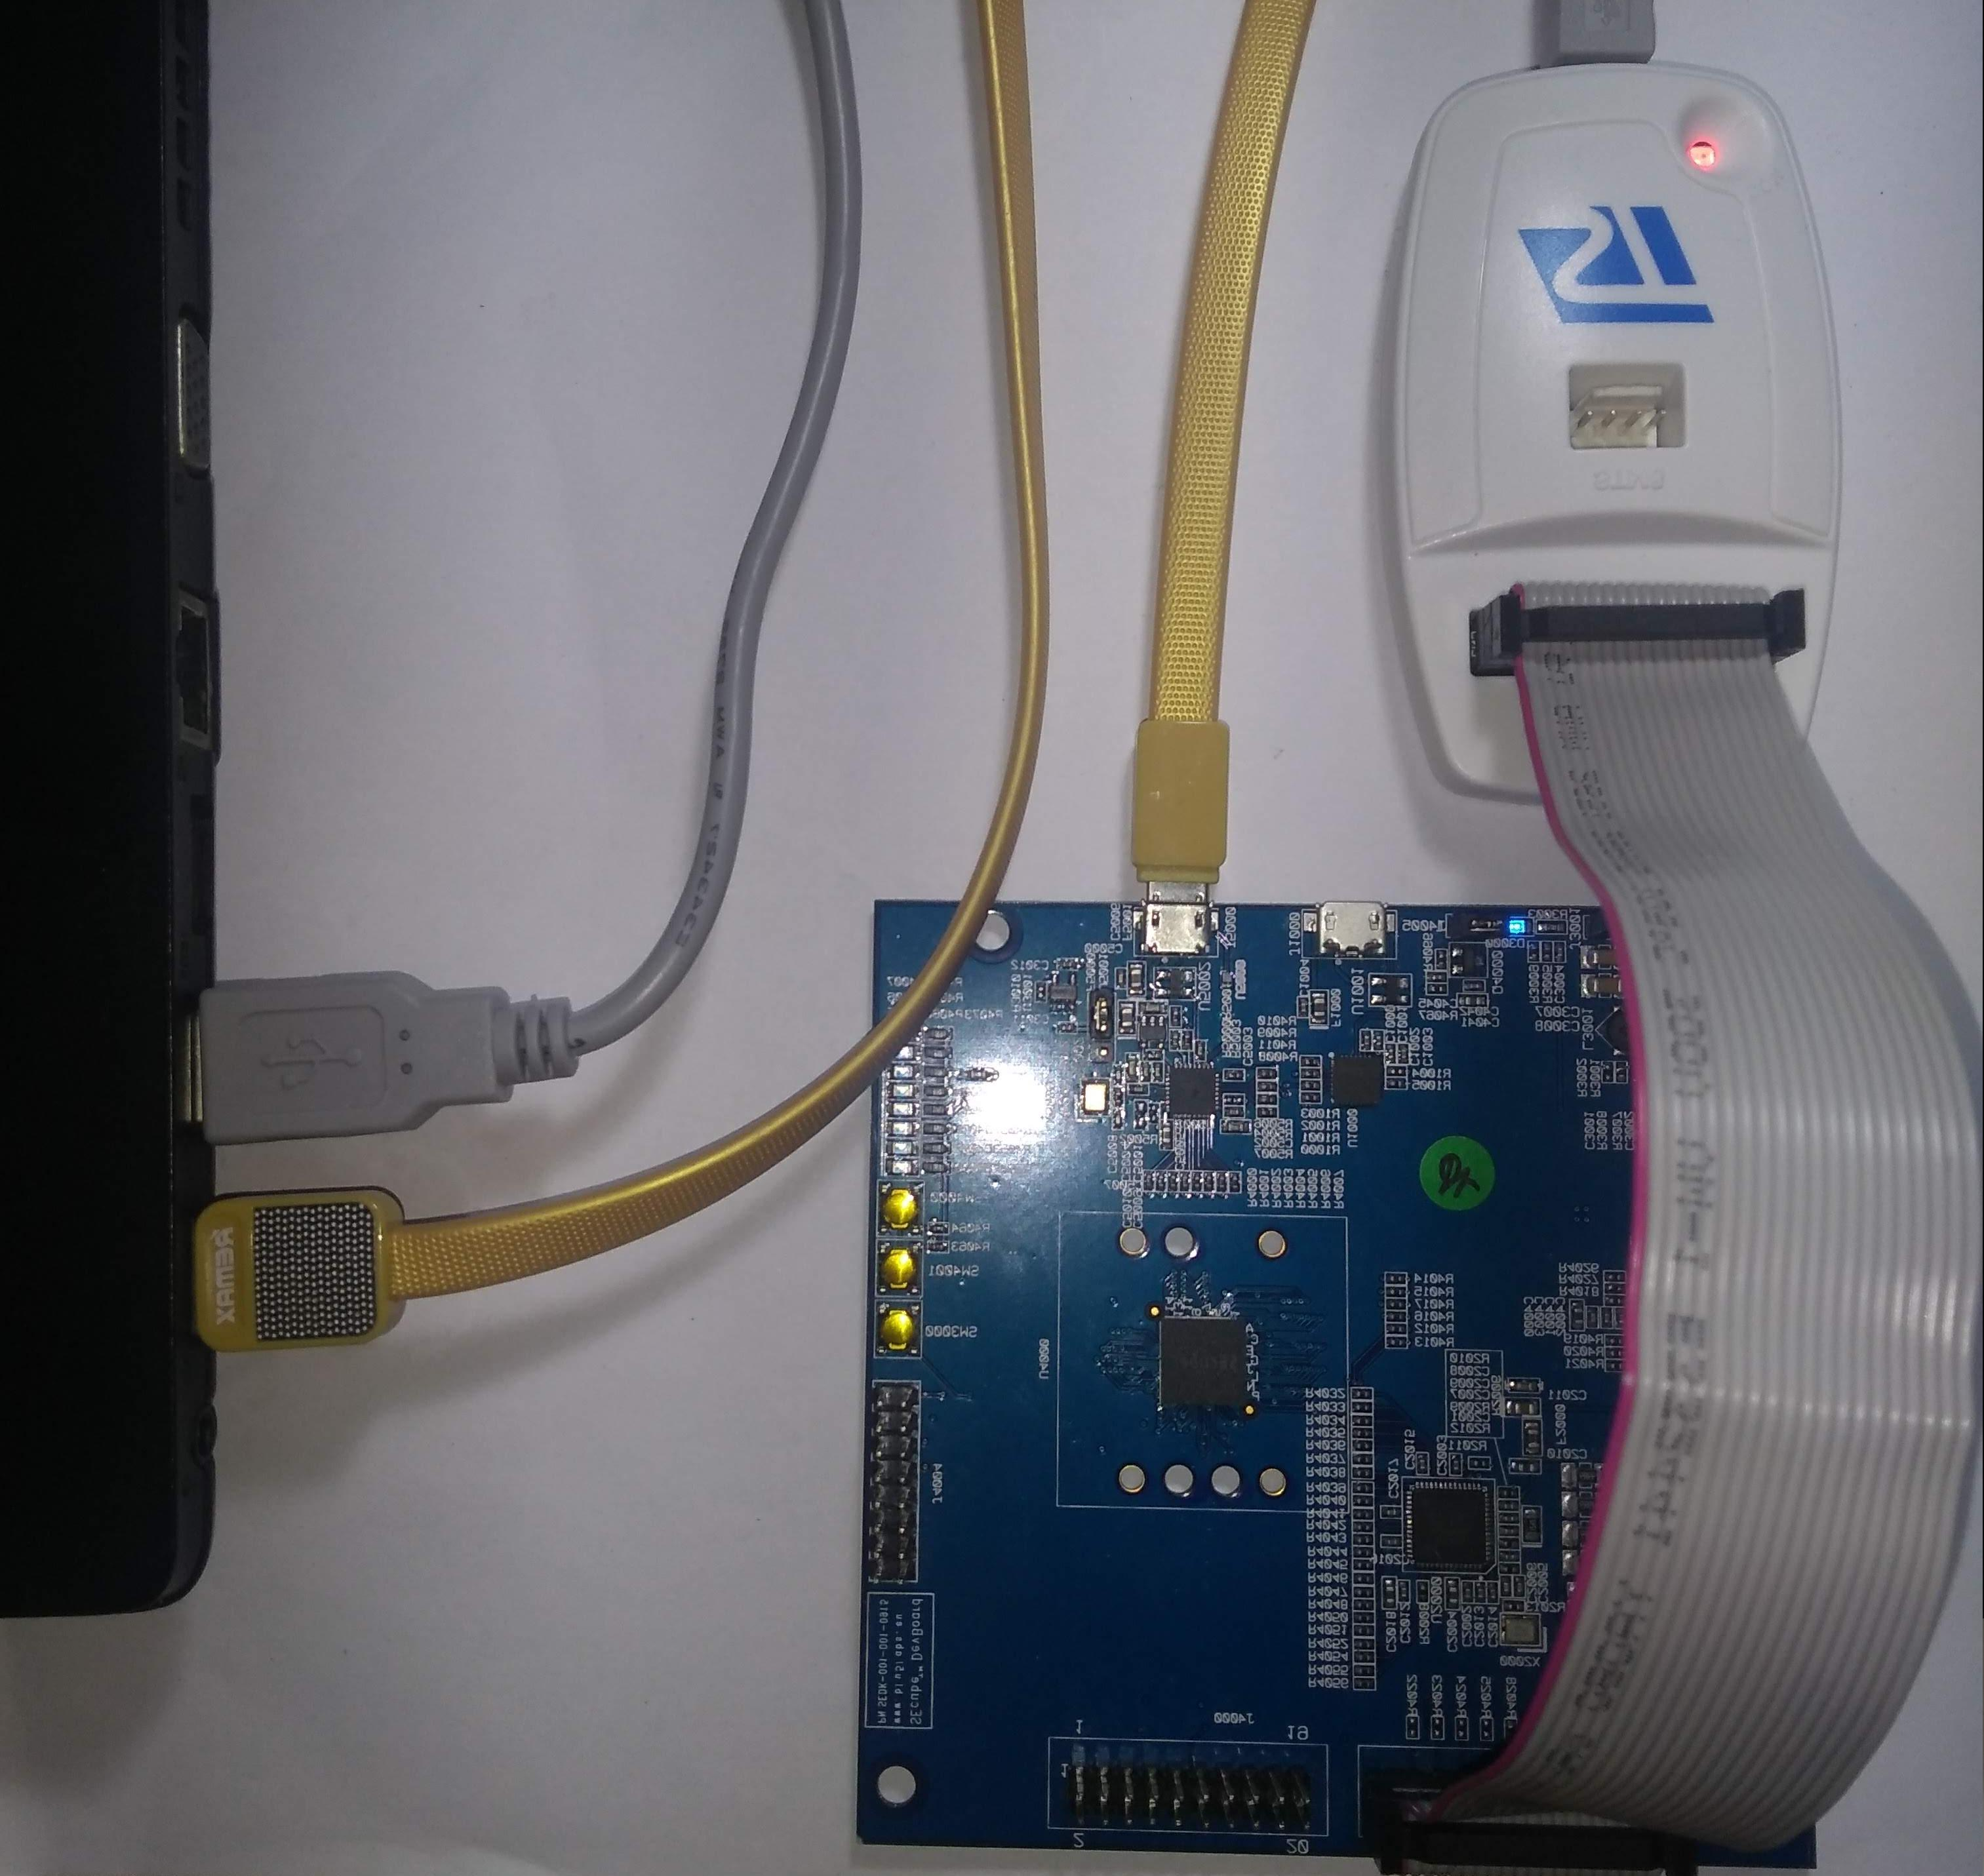
\includegraphics[width=0.48\textwidth]{chapters/figures/frameworks/conReal2}}
  \caption{DevKit and ST-Link/V2 connections to PC}
 \label{fig:con}
\end{figure}

The Getting Started guide does a very good job explaining in detail how to install all the necessary software. Here a brief recap of the followed steps is giving, plus some additional configurations that are required when running the IDE on Linux (In the author's case, Linux Mint 17.1, kernel 3.13.0-37).


\begin{enumerate}
\setlength\itemsep{0pt}
\item \textbf{Java Runtime Environment:} Necessary to run Eclipse, as it is a Java program. The version 1.8.0\_171 was installed, available at \cite{java}

\item \textbf{Eclipse:} Eclipse for C/C++, Neon version was used. Available at \cite{eclipse}

\item \textbf{AC6 Tools Eclipse Plugin: }  Embedded Toolchain for ARM, which includes the building tools (GCC-based ARM cross compiler, assembler and linker), OpenOCD (Open On-Chip Debugger) and GDB debugging tools. In Linux, OpenOCD allows the communication with the STLink-V2 and therefore, the debugging. Available at \cite{ac6}.

\item \textbf{STM32CubeMX: }This is a STM32Cube initialization code generator that includes standard toolchains and embedded software libraries and middleware components (e.g., Open-source TCP/IP stack, USB drivers, open-source FAT file system, open source RTOS). Available at \cite{cubemx}.

\item \textbf{udev rules (Linux Only): }On Linux, it is required to include the STLink-v2 device rules in the udev device manager. To do so, instead of writing them manually it is easier to use the rules already generated in the mcu-gnu-eclipse version of openocd available in \cite{mcu}. After downloading the appropriate version (*centos64.tgz for a 64 bits Linux machine), the \texttt{.tgz} file is extracted and the \texttt{60-openocd.rules} file copied into the \texttt{rules.d/} directory using the commands in listing \ref{lis:udev}:

\begin{lstlisting}[float=htb, basicstyle=\ttfamily, frame=tb, caption={Including STLink rules to udev manager in Linux}, label = {lis:udev}]
sudo cp /gnu-mcu-eclipse/openocd/0.10.0-8-20180512-1921/
contrib/60-openocd.rules  /etc/udev/rules.d/

sudo udevadm control --reload-rules
\end{lstlisting}


\item \textbf{SEcube™ Open SDK: }Finally, the Open SDK available at \cite{SEcubeRes} can be used. There is an already configured environment for development, in the zip file \texttt{SEcubeSDK\_GAF\_14gen2017/SEcube\_SDK/Development/ Environment.zip}. After extracting it, the folder \texttt{/Environment/ws} can be used as Eclipse workspace. This opens the current version of the SEcube™ firmware, that can be then modified and loaded into the chip.

\end{enumerate}




\section{PwGen: Pronounceable Password generator}

The most secure type of passwords are random ones. A random password sufficiently long is considered to be virtually unbreakable. But this rises two problems: First of all, humans are inherently bad at creating true random passwords. Second, a random password is not suited to be remembered or even used (as it probably is too annoying to type). These two reasons motivated the inclusion of a Password Generator.

pwgen is an open source program that generates human friendly passwords that are also secure. It is available in the official Linux repositories, and there is a Windows version as well, but in this work the source files where used.

``The pwgen program generates passwords which are designed to be easily memorized by humans, while being as secure as possible. Human-memorable passwords are never going to be as secure as completely completely random passwords. In particular, passwords generated by pwgen without the -s option should not be used in places where the password could be attacked via an off-line brute-force attack. On the other hand, completely randomly generated passwords have a tendency to be written down, and are subject to being compromised in that fashion'' \cite{pwgen}.

pwgen offers several options that can drastically change the type of generated password. Here is a list of the options available for users of SEcubeWallet:

\begin{itemize}
\setlength\itemsep{0pt}


\item \textbf{Length:} The desired length of the password. It is recommended to be at least 12 for non-random passwords and 8 for random ones.

\item \textbf{-0, no numerals:} 
Don't include numbers in the generated passwords. 

\item \textbf{-A, no capitalize:} 
Don't bother to include any capital letters in the generated passwords. 
    
\item \textbf{-B, ambiguous:}
Don't use characters that could be confused by the user when printed, such as 'l' and '1', or '0' or 'O'. This reduces the number of possible passwords significantly, and as such reduces the quality of the passwords. It may be useful for users who have bad vision, but in general use of this option is not recommended. 
    
\item \textbf{-c, capitalize:}
Include at least one capital letter in the password.

\item \textbf{-n, numerals:}
Include at least one number in the password.

\item \textbf{-s, secure:}
Generate completely random, hard-to-memorize passwords.

\item \textbf{-v, no vowels:}
Generate random passwords that do not contain vowels or numbers that might be mistaken for vowels. It provides less secure passwords to allow system administrators to not have to worry with random passwords accidentally contain offensive substrings. 

\item \textbf{-y, symbols:}
Include at least one special character in the password.
\end{itemize}

By default pwgen behaves as if the options \textbf{-nc} were used, that is, pronounceable passwords with at least 1 capital letter and 1 number.

The strongest passwords this program can generate are obtained with the options \textbf{-ys}, as it results in random passwords with special symbols. They are very hard to remember, and should only be used if the user is willing to open the SEcubeWallet application each time they need to use one of the password.


\section{zxcvbn: Password strength estimation} \label{sec:zxcvbnth}

An important feature to have in a password manager is the possibility to realistically estimate how strong a password is, i.e., how hard could it be for hackers to crack it, as there is no point in using the SEcube™ system to protect weak passwords, that could be easily guessed with brute force attacks. As it is out of the author expertise to write a reliable function to make this estimation, it was decided to use a trusted project developed during the dropbox hackweek event in 2012. The estimator called \textbf{zxcvbn} was originally written in JavaScript aiming for an easy integration with multiple web browsers and OS. Fortunately, the community ported the library to a wide variety of languages including Python, Ruby and C/C++. In this work the C++ implementation was used. The project is Open Source and available for free use on GitHub \cite{zxgit}.

zxcvbn is regarded by the community as one of the most reliable and mathematically advanced open source password estimators. In security forums and discussion it always pops out as an excellent tool, much better than other passwords estimators commonly used in web pages. In \cite{naked}, the author compares zxcvbn to other popular java meters and arrives to the conclusion that only zxcvbn is reliable enough to actually give an useful feedback.
In \cite{gen_est_eval}, the author makes an evaluation of several password generators and strength estimators. PwGen and zxcvbn, the two libraries used in this work, always give excellent results.

``For over 30 years, password requirements and feedback have largely remained a product of LUDS: counts of Lower- and Uppercase letters, Digits and Symbols. LUDS remains ubiquitous despite being a conclusively burdensome and ineffective security practice. zxcvbn is an alternative password strength estimator that is small, fast, and crucially no harder than LUDS to adopt. Using leaked passwords, we compare its estimations to the best of four modern guessing attacks and show it to be accurate and conservative at low magnitudes, suitable for mitigating online attacks. We find 1.5 MB of compressed storage is sufficient to accurately estimate the best-known guessing attacks up to 105 guesses, or 104 and 103 guesses, respectively, given 245 kB and 29 kB. zxcvbn can be adopted with 4 lines of code and downloaded in seconds. It runs in milliseconds and works as-is on web, iOS and Android''. \cite{zxpaper}

``People of course choose patterns — dictionary words, spatial patterns like \texttt{qwerty}, \texttt{asdf} or \texttt{zxcvbn}, repeats like \texttt{aaaaaaa}, sequences like \texttt{abcdef} or \texttt{654321}, or some combination of the above. For passwords with uppercase letters, odds are it’s the first letter that’s uppercase. Numbers and symbols are often predictable as well: \texttt{l33t} speak (3 for e, 0 for o, @ or 4 for a), years, dates, zip codes, and so on.
As a result, simplistic strength estimation gives bad advice. Without checking for common patterns, the practice of encouraging numbers and symbols means encouraging passwords that might only be slightly harder for a computer to crack, and yet frustratingly harder for a human to remember. xkcd nailed it''. (see figure \ref{fig:xkcd}). \cite{zxdropbox}

\begin{figure}[htb]
  \centering
  \captionsetup{justification=centering}
  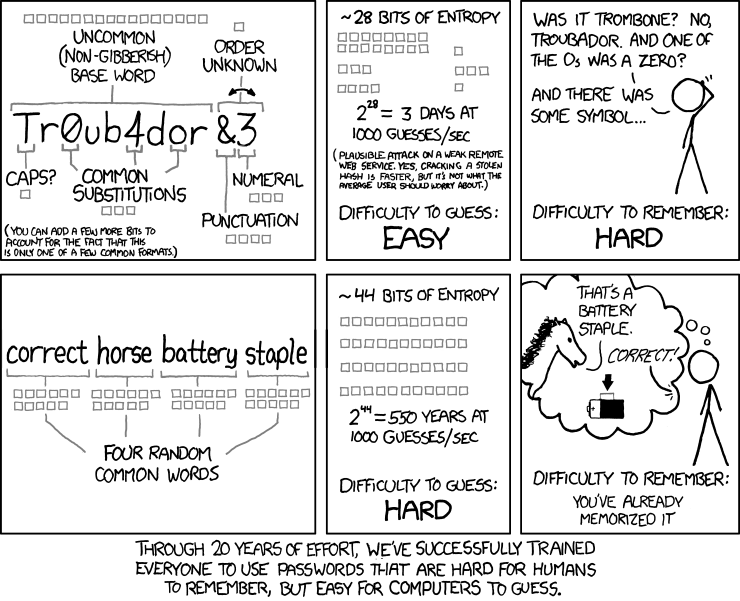
\includegraphics[width=\columnwidth]{chapters/figures/development/xkcd.png}
  \caption{Password strength, xkcd \cite{xkcd}}
  \label{fig:xkcd}
\end{figure}

To put it in other words, the authors of the project argue that a password like \texttt{correcthorsebatterystaple} (a nonsense English phrase) is more strong than a password like \texttt{Tr0ub4dour\&3}, even if the former does not have any upper cases or numbers, and the latter seems more complicated.

\begin{figure}[htb]
  \centering
  \captionsetup{justification=centering}
  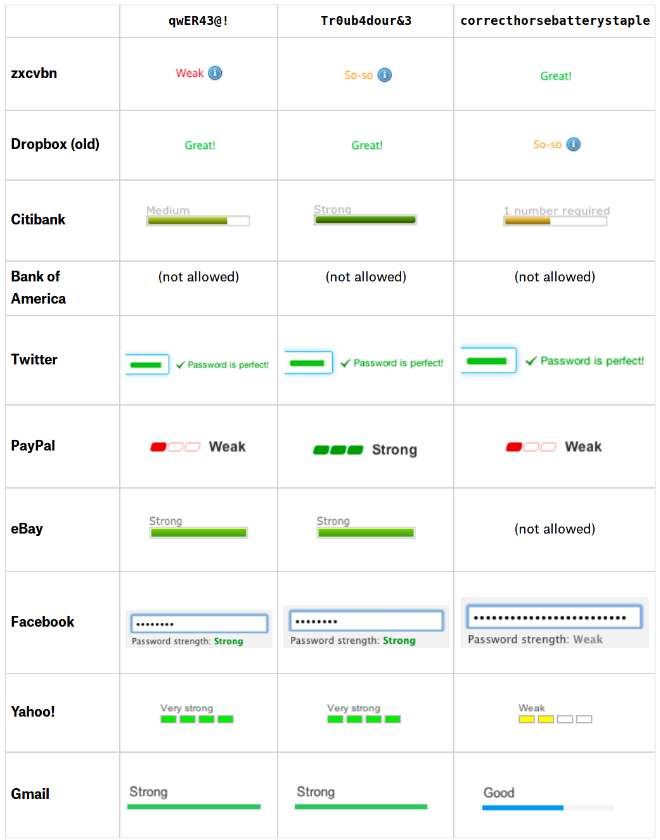
\includegraphics[width=\columnwidth]{chapters/figures/development/zxcvbn_comp.png}
  \caption{comparison between zxcvbn and popular websites' strength meters}
  \label{fig:tablez}
\end{figure}

The table in figure \ref{fig:tablez} (taken from \cite{zxdropbox}), show how zxcvbn is different from strength meters used in popular web services. (disclaimer: The data in the table is from 2012). From it we can learn:

\begin{enumerate}
\setlength\itemsep{-3pt}

\item Passwords like \texttt{\textbf{qwER43@!}}, which is a spatial password: it uses the keys \texttt{qwer4321}, with shift pressed for the keys \texttt{er} and \texttt{21} (the \texttt{@} symbol in the English keyboard is \texttt{shift+2}), is not considered week by most of the meters, but it should. It is probably due to the fact that it includes a combination of numbers and symbols that makes it look strong, but in reality, because of keyboard spatiality, is not.

\item Passwords like \texttt{\textbf{Tr0ub4dour\&3}}, which is generated by replacing some of Troubadour letters with numbers, and adding two more characters, is regarded as a very strong password for all of the meters except zxcvbn. Even if the base word is uncommon, and it has some variations, it is not long enough to be considered so strong.
\item A password like \texttt{\textbf{correcthorsebatterystaple}} is not considered strong by most of the meters except zxcvbn, and it is not even allowed in some cases because it lacks numbers, Upper-cases or symbols.
\end{enumerate}

The superiority of zxcvbn over the other meters in the table may seem like cherry picking, but the way zxcvbn is constructed explains these differences.

\subsubsection*{Matching}

Enumerates all the (possibly overlapping) patterns it can detect. Currently zxcvbn matches against:

\begin{itemize}
\setlength\itemsep{-3pt}


\item \textbf{Dictionaries:} Common words the user is likely to use as password. Multiple dictionaries, in a simple .txt format can be used. In this work, we present a few: English words, Italian words, names and surnames, Burnett’s 10,000 common passwords, words from tv and films. The match has an associated frequency rank, where words like the and good have low rank, and words like photojournalist and maelstrom have high rank. This lets zxcvbn scale the calculation to an appropriate dictionary size on the fly, because if a password contains only common words, a cracker can succeed with a smaller dictionary. For all dictionaries, match recognizes uppercasing and common \texttt{l33t} substitutions.

\item \textbf{Spatial keyboard patterns:} Some users are likely to choose passwords based on spatial pattern. For instance a user could choose the first row of letters from right to left: \texttt{poiuytrewq} as they password. \textsc{qwerty} keyboard, Dvorak keyboard, and keypad are considered.

\item \textbf{Repeats}: Users are also prone to use repetition of characters, like \texttt{rrrr}. 

\item \textbf{sequences}: Numeric or alphabetic sequences like \texttt{123} or \texttt{fedcba}

\item \textbf{years and dates}: The year or full date of a special event, like anniversary or birthday. Years from 1900 to 2019 are considered and dates in different formats. (3-13-1997, 13.3.1997, 1331997). 

\end{itemize}

\subsubsection*{Entropy calculation of a single pattern}
Depending on the type of matching, the entropy calculation is done differently, but for all the cases the idea is the same: How many different cases a hacker would have to try before guessing the pattern? For example, for the repeat case, if the user chooses \texttt{zzzzz}, as it is repeated five times, and if we assume the hacker starts by the letter a, then the number of cases would be $ N = 26 \times 5 = 130 $. (The sequence the hacker would try is: \texttt{a, b, c, d...,z, aa, bb, cc,...,...,zzzz, aaaaa, bbbbb,....zzzzz}).


As the number of possible cases can be pretty large, the entropy is not given as a raw value but as $e = log_{2}(N)$, known as the entropy bits, and in some cases as $f = log_{10}(N)$, known as the log entropy. In the example, entropy bits: $e = log_{2}(130) = 7 bits$.

The entropy bits and log entropy are related by:
\[N = 2^{e} = 10^{f}\]
\[f = e \times log_{10}(2)\]
\[e = f \times log_{2}(10)\]


\subsubsection*{Minimum entropy search of whole password}

``Given the full set of possibly overlapping matches, the algorithm finds the simplest (lowest entropy) non-overlapping sequence. For example, if the password is damnation, that could be analysed as two words, dam and nation, or as one. It’s important that it be analysed as one, because an attacker trying dictionary words will crack it as one word long before two.

zxcvbn calculates a password’s entropy to be the sum of its constituent patterns. Any gaps between matched patterns are treated as brute-force "patterns" that also contribute to the total entropy. That a password’s entropy is the sum of its parts is a big assumption. However, it’s a conservative assumption. By disregarding the "configuration entropy" — the entropy from the number and arrangement of the pieces — zxcvbn is purposely underestimating, by giving a password’s structure away for free: It assumes attackers already know the structure (for example, surname-bruteforce-keypad), and from there, it calculates how many guesses they’d need to iterate through.''\cite{zxdropbox}

\subsubsection*{From entropy bits to rank and estimated crack time} \label{sec:zxLevels}

To estimate the cracking time, it is necessary to make some assumptions about what kind of attack will be subjected the user. zxcvbn considers four possible scenarios according to the number of attempts/time the hacker can do:

\begin{enumerate}
\setlength\itemsep{-3pt}


\item \textbf{Online throttling (100 per hour):} Online attack on a service that ratelimits password authentication  attempts.
  
\item \textbf{Online no throttling (10 per second): }Online attack on a service that does not ratelimit or where an attacker has outsmarted ratelimiting.

\item \textbf{Offline slow hashing (1e4 per second): }Offline attack. assumes multiple attackers, proper user-unique salting, and a slow hash function with moderate work factor, such as bcrypt, scrypt, PBKDF2.

\item \textbf{Offline fast hashing (1e10 per second): }Offline attack with user unique salting but a fast hash function like SHA1, SHA256 or MD5. A wide range of reasonable numbers anywhere from one billion to one trillion guesses per second, depending on number of cores and machines. Ballparking at 10B per sec.

\end{enumerate}

%  0 # . (guesses < 10^3)
%
%  1 # very guessable: protection from throttled online attacks. (guesses < 10^6)
%
%  2 # somewhat guessable: protection from unthrottled online attacks. (guesses < 10^8)
%
%  3 # safely unguessable: moderate protection from offline slow-hash scenario. (guesses < 10^10)
%
%  4 # very unguessable: strong protection from offline slow-hash scenario. (guesses >= 10^10)

zxcvbn then ranks a password with a security level from 0 to 4 according to its entropy value:
\begin{itemize}
\setlength\itemsep{-3pt}

\item \textbf{Level0 if ($N<10^{3}$):} Too guessable, risky password
\item \textbf{Level1 if ($N<10^{6}$):} Very guessable, protection from throttled online attacks.
\item \textbf{Level2 if ($N<10^{8}$):} Somewhat guessable, protection from unthrottled online attacks.
\item \textbf{Level3 if ($N<10^{10}$):} Safely unguessable, moderate protection from offline slow-hash scenario.
\item \textbf{Level4 if ($N>10^{10}$):} Very unguessable: strong protection from offline slow-hash scenario

\end{itemize}
Where N is the number of possibilities a hacker would have to try for crack the password. So for instance, if the password is level 2, it could be cracked in around $10^{8}$ guesses.

For Level0 the above rule in terms of the entropy bits is $e<log_{2}(10^{3})$.
In terms of the log entropy bits, it simply is $f<3$.

The level and estimated crack time for each type of attack is presented to the user. With this information, the user will, hopefully, choose a Level4 password. Additionally, the user also receives  feedback about how the password was cracked, so they know how to improve it.

\section{PassPhrase Generator}

From the previous two sections there seems to be a disagreement on what a good password looks like. PwGen can generate totally random passwords or pseudo-random pronounceable passwords, but even the later go against what zxcvbn proposes: PassPhrases that are very easy to remember, but long enough to give excellent entropy results. To fill this gap, a PassPhrase generator that gives results along the lines of \texttt{CorrectHorseBatteryStaple} is used.

The PassPhrase generator developed by the author works by randomly picking out words from dictionary files. The user can tune the PassPhrase generation as follows:

\begin{itemize}
\setlength\itemsep{-3pt}

\item \textbf{Dictionaries: }The user must select appropriate dictionaries, containing a sufficiently large number of lines (larger than 10000) to ensure the picked words are really random. The English and Italian dictionaries used by zxcvbn are a good example. The user can work with as many dictionaries as desired, an the format must be one word per line. Only the first word of each line is counted, as everything after a space is trimmed.

\item \textbf{Number of words: }The user can configure the number of words the generated PassPhrases are composed of. The recommended size is four, but it can be as long as the user wants.

\item \textbf{Minimum Length of Words: }With this option is possible to select only random words whose length is higher than a certain value. This is to make sure the resulting PassPhrase is too short and therefore too insecure. The drawback here is that the higher the selected threshold, the fewer the available words in the dictionaries.

\item \textbf{Only use infrequent words: }If the dictionaries follow the same format as those used for zxcvbn, that is, the words are ordered by frequency, having the most uncommon words in the lower part of the dictionary, the user can then ask to generate PassPhrases containing only unusual words. The drawback here is, again, fewer words to choose from. The percentage of words that are used is configurable.

\item \textbf{Capitalize first letter: }To make the PassPhrases more readable, the first letter of each word can be capitalized.
\end{itemize}